\documentclass[../classical_mechanics.tex]{subfiles}

\begin{document}

    \section{Conservation of Momentum}\label{sec:conservation-of-momentum}
        \paragraph{}
        Consider two objects interacting with each other via some forces.
        They could be two electrons repelling each other because of the electrostatic force or two planets falling together due to gravity.
        By Newton's third law,
        % TODO: include diagram for this
        \begin{equation}
            \vec{F}_{A\to B}(t)=-\vec{F}_{B\to A}(t),
        \end{equation}
        and so by Newton's second law we can write
        \begin{equation}\label{eq-COM-acc}
            m_A\vec{a}_A(t)+m_B\vec{a}_B(t)=0.
        \end{equation}
        We can integrate this equation over some arbitrary time period $t_1<t_2$ to get
        \begin{align}
            \int_{t_1}^{t_2}\left(m_A\vec{a}_A(t)+m_B\vec{a}_B(t)\right)\dd{t}&=m_A\left(\vec{v}_A(t_2)-\vec{v}_A(t_1)\right)+m_B\left(\vec{v}_B(t_2)-\vec{v}_B(t_1)\right)\\
            &=0\\
            \implies m_A\vec{v}_A(t_1)+m_B\vec{v}_B(t_1)&=m_A\vec{v}_A(t_2)+m_B\vec{v}_B(t_2).
        \end{align}
        Thus, we have discovered that Newton's third law implies that the quantity $m_A\vec{v}_A+m_B\vec{v}_B$ is \textbf{conserved}.
        This means it is constant for all time. We call this quantity the \textbf{linear momentum}.

    \section{Centre of Mass}\label{sec:centre-of-mass}
        \paragraph{}
        Some times it is useful to consider the \textbf{centre of mass} of a system, which is defined as the \textit{average} position of all the objects in the system.
        For the system of two objects, this is calculated as
        \begin{equation}
            \vec{r}_\text{COM}=\frac{m_A\vec{r}_A+m_B\vec{r}_B}{m_A+m_B}.
        \end{equation}
        This defines a position vector which points to the centre of mass of the system.
        By differentiating this vector with respect to time, we can get the velocity of the centre of mass
        \begin{equation}
            \vec{v}_\text{COM}=\dv{\vec{r}_\text{COM}}{t}=\frac{m_A\dv{\vec{r}_A}{t}+m_B\dv{\vec{r}_B}{t}}{m_A+m_B}=\frac{m_A\vec{v}_A+m_B\vec{v}_B}{m_A+m_B}.
        \end{equation}
        This is just the total momentum of the two objects divided by their total mass, and we found before that the total momentum was conserved.
        % TODO: hint at when it is not conserved
        \begin{equation}
            (m_A+m_B)\vec{v}_\text{COM}=m_A\vec{v}_A+m_B\vec{v}_B=\text{constant}.
        \end{equation}
        From these definitions we can see that equation \ref{eq-COM-acc} is the accleration of the centre of mass multiplied by the total mass, which by Newton's second law is the force on the centre of mass.
        This implies that if the resultant force on the centre of mass is 0, then the centre of mass moves with constant velocity, just like a single object following Newton's first law, and the total linear momentum is conserved.
        \begin{example}
            For a system of two objects, show that the centre of mass is always located on the line that connects the two objects.
            % TODO: write this
        \end{example}

        \paragraph{}
        For a general system of $N$ objects, we define the total mass and total momentum as
        \begin{align}
            M&=m_1+m_2+\dots+m_N\\
            &=\sum_{i=1}^{N}m_i\\
            \vec{P}&=\sum_{i=1}^{N}m_i\vec{v_i}.
        \end{align}

        \paragraph{}
        % TODO: include diagram for this
        The net force on each individual part of the system can be written as the sum of any external forces and internal forces from all the other parts.
        \begin{equation}
            \vec{F}_{i,\text{net}}=\vec{F}_{i,\text{ext}}+\sum_{j\neq i}^N\vec{F}_{j\to i}.
        \end{equation}
        Let's now add all the forces together to get the net force on the centre of mass:
        \begin{equation}
            \vec{F}_\text{net} = \sum_{i=1}^N\vec{F}_{i,\text{net}} = \underbrace{\sum_{i=1}^N\vec{F}_{i,\text{ext}}}_{=\vec{F}_\text{ext}}+\underbrace{\sum_{i=1}^N\sum_{j\neq i}^N\vec{F}_{j\to i}}_{=0}.
        \end{equation}
        The second term on the far right-hand side is 0 by Newton's third law (you can prove this by induction).
        % TODO: write example to prove this (F_12 cancels with F_21, F_13 cancels with F_31, F_23 cancels with F_32, etc.)
        
        \paragraph{}
        Now we define the centre of mass position, velocity, and acceleration as the weighted average of each of the individual particles' quantities.
        \begin{definition}
            Consider a system of $N$ objects.
            The \textbf{centre of mass} is is a vector function defined as
            \begin{equation}
                \vec{r}_\text{COM}=\frac{1}{M}\sum_{i=1}^N m_i\vec{r}_i.
            \end{equation}
            The \textbf{centre of mass velocity} is defined as
            \begin{equation}
                \vec{v}_\text{COM}=\dv{\vec{r}_\text{COM}}{t}=\frac{1}{M}\sum_{i=1}^N m_i\dv{\vec{r}_i}{t}=\frac{1}{M}\sum_{i=1}^N m_i\vec{v}_i=\frac{\vec{P}}{M},
            \end{equation}
            and the \textbf{centre of mass acceleration} is defined as
            \begin{equation}
                \vec{a}_\text{COM}=\dv[2]{\vec{r}_\text{COM}}{t}=\frac{1}{M}\sum_{i=1}^N m_i\dv[2]{\vec{r}_i}{t}=\frac{1}{M}\sum_{i=1}^N m_i\vec{a}_i=\frac{1}{M}\sum_{i=1}^N\vec{F}_{i,\text{net}}=\frac{\vec{F}_\text{ext}}{M},
            \end{equation}
        \end{definition}
        Notice that in the definition of centre of mass acceleration, we have shown that
        \begin{equation}\label{eq-NII-macroscopic}
            M\vec{a}_\text{COM}=\vec{F}_\text{ext}.
        \end{equation}
        This result is actually quite profound because it is what allows us to treat systems of particles as point masses themselves while ignoring all of the internal forces between the particles since they all cancel out.
        Also note that because the centre of mass momentum is equal to the total momentum, systems of many particles act as if all the mass was concentrated in a point at the centre of mass, moving with the the centre of mass velocity.
        Without these results, we could not apply the laws of mechanics as we have been learning them to macroscopic bodies!

        \paragraph{}
        If $\vec{F}_\text{ext}=0$, i.e. the system is isolated and there are no external forces, then the centre of mass moves in a straight line with a constant velocity and the total linear momentum is conserved.
        % TODO: write example of a projectile exploding while in the air with the COM following the trajectory 

        \paragraph{}
        Since the centre of mass quantites are vectors, we can break them into components just like all the other vector quantites we have seen.
        For example, in 2D cartesian coordinates we have
        \begin{equation}
            \vec{r}_\text{COM}=\frac{1}{M}\sum_{i=1}^N m_i\vec{r}_i=\frac{1}{M}\sum_{i=1}^N m_i(x_i\ihat+y_i\jhat)=\frac{1}{M}\sum_{i=1}^N m_ix_i\ihat+\frac{1}{M}\sum_{i=1}^N m_iy_i\jhat,
        \end{equation}
        so we can define the weighted average along the $x$ and $y$ axes:
        \begin{equation}
            \vec{r}_\text{COM}=\bar{x}\ihat+\bar{y}\jhat,\quad\bar{x}=\frac{1}{M}\sum_{i=1}^N m_ix_i,\quad\bar{y}=\frac{1}{M}\sum_{i=1}^N m_iy_i
        \end{equation}

    \section{Continuous Extended Objects}\label{sec:continuous-extended-objects}
        \paragraph{}
        In the case where the number of particles in the system becomes so large that the distinction between the individual particles becomes smooth, we stop computing the centre of mass quantities as discrete sums and switch to integrals.
        The intuition for this is as follows.
        As the number of particles $N$ tends to infinity, the mass $m_i$ becomes a small mass element $\dd{m}$, which is what we integrate over.
        \begin{equation}
            M=\int\dd{m},\quad\vec{r}_\text{COM}=\frac{1}{M}\int\vec{r}\dd{m}.
        \end{equation}
        To evaluate this integral, we will need to convert the mass element $\dd{m}$ into a spatial element, for example a length, area, or volume element.
        This is done using a linear, surface, or volume density.
        \begin{equation}
            \dd{m}=\lambda(x)\dd{x},\quad\dd{m}=\sigma(\vec{r})\dd{A},\quad\dd{m}=\rho(\vec{r})\dd{V}.
        \end{equation}

        \paragraph{}
        We will look at some examples here in the form of uniform lamina, which are flat (two-dimensional) extended objects with uniform surface density.
        \begin{example}
            Find the centre of mass of a right triangle with both small side lengths $a$.
            \begin{figure}[H]
                \centering
                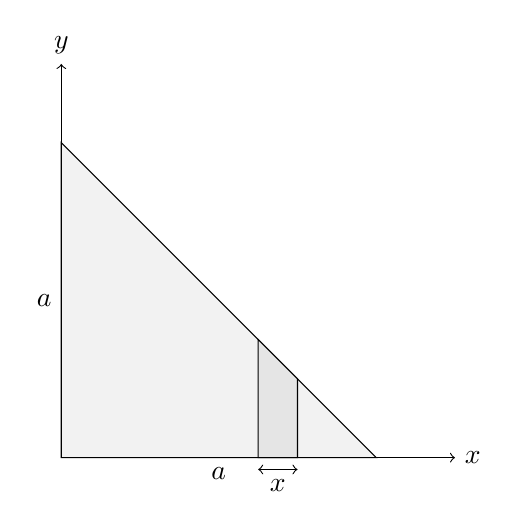
\begin{tikzpicture}[scale=5]
                    \draw[<->] (0,1) |- (1,0);
                    \node[above] at (0,1) {$y$};
                    \node[right] at (1,0) {$x$};

                    \filldraw[fill=black!5] (0,0) -- (0,0.8) -- (0.8,0) -- cycle;
                    \node[below] at (0.4,0) {$a$};
                    \node[left] at (0,0.4) {$a$};

                    \filldraw[fill=black!10] (0.5,0) -- (0.6,0) -- (0.6,0.2) -- (0.5,0.3) -- cycle;
                    \draw[<->] (0.5,-0.03) -- (0.6,-0.03);
                    \node[below] at (0.55,-0.03) {$\dd{x}$};
                \end{tikzpicture}
            \end{figure}
            
            \paragraph{}
            We will find each component of the centre of mass position separately.
            In fact, by the symmetry of the shape we only need to find the average $x$ position, because the average $y$ position will be the same.
            We will break the triangle up into thin vertical slices of area $y\dd{x}$.
            Note that $y=a-x$ (equation of a straight line), so we have
            \begin{equation}
                \bar{x}=\frac{1}{M}\int x\dd{m}=\frac{1}{M}\int_0^a\sigma xy\dd{x}=\frac{1}{M}\int_0^a\sigma x(a-x)\dd{x}.
            \end{equation}
            The total mass of the uniform lamina is $M=\frac{1}{2}\sigma a^2$, so the integral becomes
            \begin{equation}
                \bar{x}=\frac{2}{a^2}\int_0^a(ax-x^2)\dd{x}=\frac{2}{a^2}\left[\frac{ax^2}{2}-\frac{x^3}{3}\right]_0^a=\frac{a}{3}.
            \end{equation}
            Thus the centre of mass position is $\vec{r}_\text{COM}=\left(\frac{a}{3},\frac{a}{3}\right)$.
        \end{example}
        \begin{example}
            Find the centre of mass of a hemicircular uniform lamina of radius $r$.
            \begin{figure}[H]
                \centering
                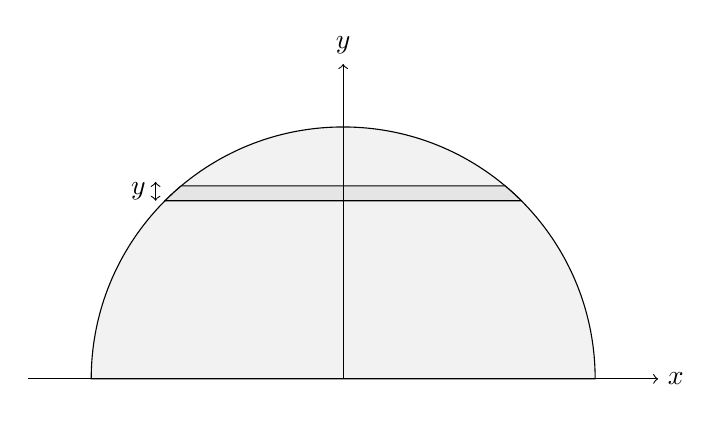
\begin{tikzpicture}[scale=4]
                    \filldraw[fill=black!5] (0.8,0) arc [radius=0.8, start angle=0, end angle=180] -- cycle;
                    \filldraw[fill=black!10] (45:0.8) arc (45:50:0.8) -- (130:0.8) arc (130:135:0.8) --cycle;
                    \begin{scope}[shift={(135:0.8)}, scale=0.06]
                        \draw[<->] (-0.5,0) -- (-0.5,1);
                        \node[left] at (-0.5,0.5) {$\dd{y}$};
                    \end{scope}

                    \draw[->] (0,0) -- (0,1);
                    \draw[->] (-1,0) -- (1,0);
                    \node[above] at (0,1) {$y$};
                    \node[right] at (1,0) {$x$};
                \end{tikzpicture}
            \end{figure}

            \paragraph{}
            By symmetry, we can see that $\bar{x}$ must be zero.
            Then, dividing the lamina into horizontal slices of area $2x\dd{y}$ (remember the factor of two because the slice goes from negative $x$ to positive $x$!), and using the equation of a circle to write $x=\sqrt{r^2-y^2}$, we get
            \begin{equation}
                \bar{y}=\frac{1}{M}\int y\dd{m}=\frac{1}{M}\int_0^r2\sigma xy\dd{y}=\frac{1}{M}\int_0^r2\sigma y\sqrt{r^2-y^2}\dd{y}.
            \end{equation}
            The total mass of the hemicircle is $M=\frac{1}{2}\sigma\pi r^2$, so
            \begin{equation}
                \bar{y}=\frac{4}{\pi r^2}\int_0^ry\sqrt{r^2-y^2}\dd{y}=\frac{4r}{3\pi}.
            \end{equation}
            The center of mass is therefore $\vec{r}_\text{COM}=\left(0,\frac{4r}{3\pi}\right)$.
        \end{example}
        \begin{example}
            Sometimes we can solve the problem using symmetries without having to do any integrals at all.
            Consider the following uniform lamina.
            \begin{figure}[H]
                \centering
                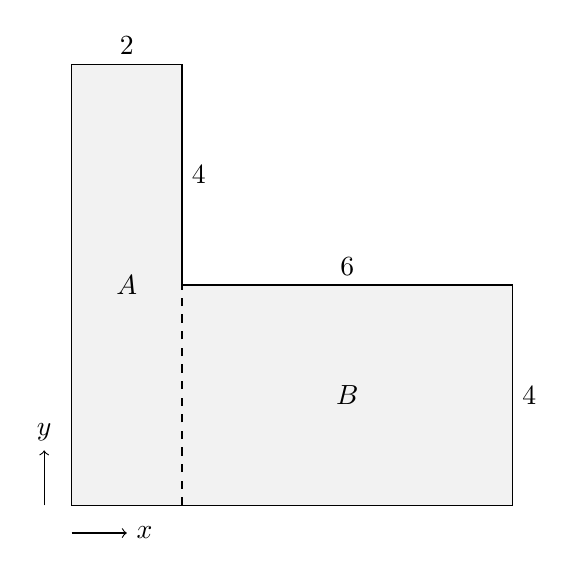
\begin{tikzpicture}[scale=0.7]
                    % TODO: add crosses for centre of masses
                    \filldraw[fill=black!5] (0,0) -- (8,0) -- (8,4) -- (2,4) -- (2,8) -- (0,8) -- cycle;
                    \draw[dashed] (2,0) -- (2,4);

                    \draw[->] (0,-0.5) -- (1,-0.5);
                    \node[right] at (1,-0.5) {$x$};
                    \draw[->] (-0.5,0) -- (-0.5,1);
                    \node[above] at (-0.5,1) {$y$};

                    \node[above] at (1,8) {$2$};
                    \node[above] at (5,4) {$6$};
                    \node[right] at (2,6) {$4$};
                    \node[right] at (8,2) {$4$};

                    \node at (1,4) {$A$};
                    \node at (5,2) {$B$};
                \end{tikzpicture}
            \end{figure}
            Using the techniques we have built up in this chapter, we can find the centre of mass without doing any integrals.

            \paragraph{}
            Firstly, we can consider the whole object in two separate subsections.
            We will call the left section $A$ and the right section $B$.
            Then the centre of mass of the whole lamina will be the average of the centres of mass of each subsection.
            \begin{equation}
                \vec{r}_\text{COM}=\left(\frac{m_A x_{\text{COM},A}+m_B x_{\text{COM},B}}{m_A+m_B},\frac{m_A y_{\text{COM},A}+m_B y_{\text{COM},B}}{m_A+m_B}\right)
            \end{equation}
            Since both subsections are rectangles, by symmetry the centre of mass must be the geometric centre.
            Thus, the centre of mass of section $A$ is $(1,4)$ and for section $B$ it is $(5,2)$.
            Now, we need to know the mass of each subsection.
            Note that since the surface density is uniform, the mass is proportional to area.
            So the mass of section $A$ is proportional to the area of section $A$, likewise for section $B$, and the total mass is proportional to the total area.
            \begin{equation}
                m_A\propto A_A,\quad m_B\propto A_B,\quad m_A+m_B\propto A_A+A_B.
            \end{equation}
            The area of section $A$ is $16$ square units, and the area of section $B$ is $24$ square units, so now we can calculate the ratios of mass of subsection to total mass:
            \begin{equation}
                \frac{m_A}{m_A+m_B}=\frac{A_A}{A_A+A_B}=\frac{16}{40}=\frac{2}{5},\quad\frac{m_B}{m_A+m_B}=\frac{A_B}{A_A+A_B}=\frac{24}{40}=\frac{3}{5}.
            \end{equation}
            Therefore, the centre of mass of the whole lamina is
            \begin{equation}
                \vec{r}_\text{COM}=\left(\frac{2}{5}1+\frac{3}{5}5,\frac{2}{5}4+\frac{3}{5}2\right)=(3.4,2.8).
            \end{equation}
        \end{example}

    \section{Impulse}\label{sec:impulse}
        \paragraph{}
        We have seen that an object has a linear momentum given by $\vec{p}=m\vec{v}$.
        How does the momentum change under the action of a force?
        Notice that
        \begin{equation}
            \dv{\vec{p}}{t}=\dv{}{t}m\vec{v}=m\vec{a}=\vec{F},
        \end{equation}
        so we have a new way to write Newton's second law.
        % TODO: remark that this is actually a more general version of F=ma
        Let's now integrate this equation over an arbitrary time interval:
        \begin{align}
            \int_{t_1}^{t_2}\dv{\vec{p}}{t}\dd{t}&=\vec{p}(t_2)-\vec{p}(t_1)\\
            &=\Delta\vec{p}=\int_{t_1}^{t_2}\vec{F}(t)\dd{t}.
        \end{align}
        We call the integral of a force over a time interval the \textbf{impulse}.
        \begin{definition}
            The \textbf{impulse} of a force $\vec{F}$ over a time interval $t_1\leq t_2$ is defined as
            \begin{equation}
                \vec{J}=\int_{t_1}^{t_2}\vec{F}(t)\dd{t}.
            \end{equation}
            It has units of Newton second (N$\cdot$s). As we have seen, the impulse is equal to the change in momentum.
            \begin{equation}
                \Delta\vec{p}=\vec{J}.
            \end{equation}
            This result is sometimes called the \textbf{impulse-momentum theorem}.
        \end{definition}

        \paragraph{}
        If we had a constant force, then the impulse would be $\vec{J}=\vec{F}\Delta t$ ($\Delta t=t_2-t_1$).
        In most problems we want to solve this will not be the case. However, we can define the \textbf{average force} such that
        \begin{equation}
            \vec{J}=\int_{t_1}^{t_2}\vec{F}(t)\dd{t}=\vec{F}_\text{avg}\Delta t.
        \end{equation}
        % TODO: add figure to illustrate this
        This is quite useful because if we have a short interaction, we can simply consider the average force over the interval which is a good approximation.

        \paragraph{}
        For a general system of $N$ objects, the total impulse on the system over a time interval is
        \begin{equation}
            \vec{J}=\int_{t_1}^{t_2}\sum_{i=1}^N\vec{F}_i(t)\dd{t}t=\int_{t_1}^{t_2}\vec{F}_\text{ext}\dd{t}.
        \end{equation}
        By equation \ref{eq-NII-macroscopic} in the previous section,
        \begin{align}
            \vec{J}=\int_{t_1}^{t_2}\vec{F}_\text{ext}\dd{t}&=\int_{t_1}^{t_2}M\vec{a}_\text{COM}\dd{t}\\
            &=M\vec{v}_\text{COM}(t_2)-M\vec{v}_\text{COM}(t_1)\\
            &=\sum_{i=1}^N\left(m_i\vec{v}_i(t_2)-m_i\vec{v}_i(t_1)\right)\\
            &=\sum_{i=1}^N\left(\vec{p}_i(t_2)-\vec{p}_i(t_1)\right)\\
            &=\vec{P}(t_2)-\vec{P}(t_1)=\Delta\vec{P},
        \end{align}
        where $\vec{P}$ denotes the total momentum of the system.
        So the impulse-momentum theorem still holds for composite systems.
        \begin{example}
            Consider a baseball of mass $m=$0.3kg being thrown at a speed of 15ms$^{-1}$.
            If the batter bats the ball at a speed of 25ms$^{-1}$ and the bat is in contact with the ball for 0.005s, what is the impulse imparted to the ball?
            What is the average force exerted on the ball? What is the average acceleration of the ball?
            % TODO: write this example and change it to tennis
        \end{example}
        % TODO: write another example with the same impulse but much longer time interval (crumple zones?)

    \section{Transforming Between Reference Frames}\label{transforming-between-reference-frames}
        \paragraph{}
        To transform between one frame of reference to another, we subtract the constant velocity between the frames from the position vector.
        \begin{equation}
            \vec{r}^\prime(t)=\vec{r}(t)-Vt.
        \end{equation}
        We can then transform the velocity and acceleration as
        \begin{align}
            \vec{v}^\prime(t)&=\dv{\vec{r}^\prime(t)}{t}=\dv{\vec{r}(t)}{t}-V=\vec{v}(t)-V\\
            \vec{a}^\prime(t)&=\dv[2]{\vec{r}^\prime(t)}{t}=\dv[2]{\vec{r}(t)}{t}=\vec{a}(t).
        \end{align}
        % TODO: put these in a definition?

        \paragraph{}
        One of the most useful reference frames to transform into is the centre of mass frame.

\end{document}
